% Cryptographic Soundness of a SNARK-Gated Policy Contract
%
% A focused whitepaper that traces the authorisation-soundness
% claim of the simplest SEP-style policy contract — "any current
% member admits" — down to base cryptographic assumptions, via a
% compositional reduction.
%
% Build:  make           → main.pdf
%         make clean

\documentclass[11pt,a4paper]{article}

% ─── Packages ────────────────────────────────────────────────────────
\usepackage[utf8]{inputenc}
\usepackage[T1]{fontenc}
\usepackage[margin=1in]{geometry}
\usepackage{microtype}
\usepackage{amsmath,amssymb,amsthm}
\usepackage{mathtools}
\usepackage{booktabs}
\usepackage{tabularx}
\usepackage{tikz}
\usetikzlibrary{positioning,arrows.meta,shapes.geometric,fit,calc}
\usepackage{xcolor}
\usepackage{cite}
\usepackage{url}
\usepackage[hidelinks]{hyperref}
\usepackage{cleveref}
\usepackage{parskip}

% Slightly tighter line spacing for a denser whitepaper feel.
\linespread{1.05}

% ─── Theorem environments ───────────────────────────────────────────
% Each environment gets its own counter so cleveref can label cross-
% references correctly (e.g. \Cref{lem:kzg} prints "Lemma 1", not
% "Theorem 1").
\theoremstyle{plain}
\newtheorem{theorem}{Theorem}
\newtheorem{lemma}{Lemma}
\newtheorem{proposition}{Proposition}
\newtheorem{corollary}{Corollary}

\theoremstyle{definition}
\newtheorem{definition}{Definition}
\newtheorem{assumption}{Assumption}
\newtheorem{remark}{Remark}

% Cleveref name overrides (capital and lowercase forms).
\crefname{theorem}{Theorem}{Theorems}
\Crefname{theorem}{Theorem}{Theorems}
\crefname{lemma}{Lemma}{Lemmas}
\Crefname{lemma}{Lemma}{Lemmas}
\crefname{proposition}{Proposition}{Propositions}
\Crefname{proposition}{Proposition}{Propositions}
\crefname{corollary}{Corollary}{Corollaries}
\Crefname{corollary}{Corollary}{Corollaries}
\crefname{definition}{Definition}{Definitions}
\Crefname{definition}{Definition}{Definitions}
\crefname{assumption}{Assumption}{Assumptions}
\Crefname{assumption}{Assumption}{Assumptions}
\crefname{remark}{Remark}{Remarks}
\Crefname{remark}{Remark}{Remarks}

% ─── Macros ─────────────────────────────────────────────────────────
\newcommand{\Fr}{\mathbb{F}_r}
\newcommand{\Fp}{\mathbb{F}_p}
\newcommand{\GG}{\mathbb{G}}
\newcommand{\GT}{\mathbb{G}_T}
\newcommand{\Gone}{\mathbb{G}_1}
\newcommand{\Gtwo}{\mathbb{G}_2}
\newcommand{\Cg}{C_g}
\newcommand{\Cgp}{{C_g^{\prime}}}
\newcommand{\RMem}{\mathsf{R}_{\mathsf{Mem}}}
\newcommand{\RUpd}{\mathsf{R}_{\mathsf{Upd}}}
\newcommand{\sep}[1]{\texttt{sep-#1}}
\newcommand{\negl}{\mathsf{negl}}
\newcommand{\Hash}{\mathsf{H}}
\newcommand{\Poseidon}{\mathsf{Poseidon2}}
\newcommand{\Adv}{\mathcal{A}}
\newcommand{\Setup}{\mathsf{Setup}}
\newcommand{\Prove}{\mathsf{Prove}}
\newcommand{\Verify}{\mathsf{Verify}}
\newcommand{\Commit}{\mathsf{Commit}}
\newcommand{\Open}{\mathsf{Open}}
\newcommand{\concat}{\mathbin{\|}}
\newcommand{\Empty}{\mathsf{EMPTY}}
\newcommand{\WriteLeaf}{\mathsf{WriteLeaf}}
\newcommand{\LeafIndex}{\mathsf{LeafIndex}}

% ─── Title block (brand-neutral, no author) ──────────────────────────
\title{Cryptographic Soundness of a SNARK-Gated Policy Contract:\\
       A Compositional Proof Sketch for the \texttt{sep-anarchy} Setting}

\author{}
\date{}

% ─── Document ────────────────────────────────────────────────────────
\begin{document}
\maketitle

\begin{abstract}
We give a compositional proof sketch for the authorisation
soundness of the simplest membership-policy smart contract in a
SNARK-gated group registry: \sep{anarchy}, in which any current
group member may admit a new one. The contract sits on top of a
fixed cryptographic stack --- the BLS12-381 curve, the KZG
polynomial-commitment scheme, the Poseidon2 algebraic hash, a
binary Merkle commitment to the membership set, the Fiat--Shamir
transform, and a simulation-extractable PLONK proof system ---
with each layer contributing a single concrete soundness
reduction. The update relation is defined so that an admission
requires \emph{two} Merkle witnesses --- one for the admitter's
own membership, one for the target slot's emptiness --- and
forbids overwriting the admitter's slot. We make every reduction
explicit and trace the contract's authorisation claim down to
four base assumptions: the $d$-strong Bilinear Diffie--Hellman
($d$-SBDH) problem on BLS12-381, collision resistance of the
Poseidon2 permutation under its published parameters, the
random-oracle modelling of Poseidon2 inside the Fiat--Shamir
transcript, and the one-honest-contributor assumption of the
reused structured reference string. The result is a
self-contained checklist of what must hold for the contract to
be sound, and a precise statement of what fails first under a
cryptographically-relevant quantum computer.
\end{abstract}

\section{Introduction}
\label{sec:intro}

A growing class of smart contracts replaces application-layer
trust with a single algebraic check: the contract accepts a
state-changing transaction if and only if the transaction carries
a succinct non-interactive proof that the proposed state change
is well-formed under a published relation. The proof is verified
on chain; the contract never needs to see the prover's witness.

We focus on a concrete instance of this pattern: a group
registry that maintains a public commitment $\Cg$ to a membership
set and transitions $\Cg \mapsto \Cgp$ only when accompanied by a
PLONK~\cite{gabizon-2019-plonk} proof of a fixed update relation
$\RUpd$. The relation embeds a \emph{policy predicate} that
constrains which witnesses are admissible; a small family of
policy contracts ships in production, each compiling to a
distinct $\RUpd$ instance. The simplest member of the family is
\sep{anarchy}: \emph{any current member admits any new member,
without quorum, founder set, or admin override}. We restrict our
attention to this policy throughout. Its $\RUpd$ circuit is the
smallest in the family and the easiest to reason about; results
for the other four policies follow by replacing the predicate.

\paragraph{Contribution.} We make every link in the soundness
chain explicit. For each cryptographic layer between the
on-chain authorisation check and a base hardness assumption, we
state a single reduction lemma; we then compose them into the
top-level soundness theorem. This gives a self-contained
checklist of what must hold for the contract to be sound, and a
precise statement of what fails first --- and what survives ---
under a cryptographically-relevant quantum computer.

\paragraph{Scope.} The paper covers cryptographic soundness
only. We do not analyse the contract family's governance
semantics, the messaging layer that sits above the registry, or
the broader economic or operational properties of any
deployment. Each layer of the stack has an established body of
results behind it; we cite the original constructions rather
than reproving them, and present only the composition.

\paragraph{Outline.} \Cref{sec:system} fixes the stack and the
contract. \Cref{sec:threat} states the threat model.
\Cref{sec:defs} gives the formal definitions. \Cref{sec:reductions}
presents the layer-by-layer reductions, \Cref{sec:theorem} composes
them into the top-level soundness statement. \Cref{sec:pq}
addresses post-quantum security. \Cref{sec:notes} catalogues the
implementation discipline the proof depends on.

\section{System overview}
\label{sec:system}

The registry is parameterised by a fixed cryptographic stack;
each layer below is consumed by exactly one layer above (and the
contract sits on top of them all). We summarise each layer here
and refer to the originating literature.

\paragraph{Curve --- BLS12-381.}
A pairing-friendly elliptic curve in the Barreto--Lynn--Scott
family with embedding degree $k=12$ and a 381-bit base
field~\cite{bowe-2017-bls12381}. We work with its two prime-order
subgroups $\Gone, \Gtwo$, the target group $\GT \subset
\Fp^{12}$, the bilinear non-degenerate pairing
$e \colon \Gone \times \Gtwo \to \GT$, and the scalar field
$\Fr$. The 2016 Kim--Barbulescu extended tower number-field
sieve~\cite{kim-barbulescu-2016} fixed the conservative
classical-security target at roughly 120--128 bits.

\paragraph{Polynomial commitment --- KZG.}
The pairing-based polynomial commitment scheme of Kate,
Zaverucha, and Goldberg~\cite{kate-2010-kzg}. A commitment $[f]_1
\in \Gone$ to a polynomial $f \in \Fr[X]$ of degree at most $d$
is a single $\Gone$ element, and an opening at any evaluation
point $z$ is a single $\Gone$ element. Verification is one
pairing check against a structured reference string
$\{[\tau^i]_1, [\tau^i]_2\}_{i=0}^{d}$, where $\tau \in \Fr$ is
the trapdoor.

\paragraph{Algebraic hash --- Poseidon2.}
A sponge-mode hash over $\Fr$ built from a substitution--%
permutation network with $\alpha$-power S-boxes and an MDS linear
layer~\cite{grassi-2023-poseidon2}, refining the original Poseidon
construction~\cite{grassi-2021-poseidon}. We use the canonical
$t=3$ rate-2 / capacity-1 instance with $\alpha = 5$, $R_F = 8$
full rounds, and $R_P = 56$ partial rounds; the round constants
and MDS matrix are the published canonical set.

\paragraph{Membership commitment --- Merkle tree.}
A binary Merkle tree~\cite{merkle-1989-tree} whose internal nodes
are Poseidon2 compressions of their two children. The leaf at
position $i$ encodes a member's identity commitment; the tree's
root is the public group commitment $\Cg$. An authentication
path consists of the sibling hash at every level between the
target leaf and the root.

\paragraph{NIZK transform --- Fiat--Shamir.}
The standard transform of Fiat and
Shamir~\cite{fiat-shamir-1986} that converts a public-coin
interactive proof into a non-interactive one by replacing each
verifier challenge with the hash of the transcript so far. The
hash is Poseidon2; the transcript is opened with a
relation-specific and circuit-binding domain tag, and every
public input is absorbed before any verifier challenge is drawn.
The modern multi-round security analysis is due to Don, Fehr,
Majenz, and Schaffner~\cite{don-2019-fiat-shamir}.

\paragraph{Proof system --- PLONK.}
A universal-updatable preprocessing SNARK for arithmetic
circuits over $\Fr$~\cite{gabizon-2019-plonk}, with polynomial
commitments via KZG and challenges drawn via Fiat--Shamir. Proofs
are constant-size at roughly seven hundred bytes; verification is
one pairing plus a multi-scalar multiplication. The
universal-updatable setup means that the same structured
reference string supports every circuit in the family; the
deployment reuses the SRS produced by the Ethereum Foundation KZG
Summoning Ceremony~\cite{eth-kzg-ceremony}, with provenance
pinned via SHA-256~\cite{nist-fips-180-4} into the
verifying-key supply chain.

\paragraph{On-chain verifier --- Stellar Soroban.}
The PLONK verifier is implemented as a Soroban smart contract on
Stellar, calling host functions for BLS12-381 group operations
and pairings~\cite{stellar-cap-0059} and for Poseidon and
Poseidon2~\cite{stellar-cap-0075}. The contract is policy-shaped:
one contract per SEP, each holding the verifying key for the
$\RUpd$ circuit specialised to its policy predicate.

\paragraph{The policy contract --- \sep{anarchy}.}
The on-chain contract for \sep{anarchy} accepts a transaction
$(\Cgp, \pi)$ and proceeds as follows. It checks that the public
input encoded in $\pi$ matches its currently-stored root $\Cg$;
it calls the on-chain PLONK verifier with the verifying key for
the \sep{anarchy} $\RUpd$ circuit; if verification succeeds, it
overwrites $\Cg \mapsto \Cgp$ in storage, increments an epoch
counter, and emits an admission event. The policy predicate
embedded in the $\RUpd$ circuit is the minimum that a meaningful
admission rule can be: the prover must know a valid
authentication path to some leaf in $\Cg$.

\section{Threat model}
\label{sec:threat}

We adopt a standard SNARK adversary. The adversary $\Adv$ is a
probabilistic polynomial-time algorithm. It is given the full
public state of the system: the verifying keys for every
policy's $\RUpd$ circuit, the current group commitment $\Cg$,
the epoch counter, every event emitted to date, and the full
structured reference string $\{[\tau^i]_1, [\tau^i]_2\}_{i=0}^{d}$
(the SRS is public --- only the trapdoor $\tau$ is secret).
$\Adv$ has read-only access to all prior transactions and may
mount any classical attack consistent with these capabilities.

$\Adv$ wins if it produces a transaction $(\Cgp_{\star}, \pi_{\star})$
that the on-chain verifier accepts, and such that
$\Cgp_{\star}$ is not the result of inserting a leaf into $\Cg$
under any opening of a current member's witness. Informally:
$\Adv$ wins if and only if the contract accepts an unauthorised
state change.

Soundness is the negation of this win condition --- no such
$\Adv$ exists, except with negligible probability in the
security parameter.

\section{Definitions}
\label{sec:defs}

We fix a security parameter $\lambda$ implicit in the curve and
hash choices.

\begin{definition}[Group commitment]
A \emph{group commitment} $\Cg \in \Fr$ is the Merkle root of a
binary tree of depth $D$ whose leaves are field elements, hashed
at every internal node by Poseidon2. The membership set has
cardinality at most $2^{D}$.
\end{definition}

\begin{definition}[Membership relation $\RMem$]
\label{def:rmem}
The relation
\[
\RMem
= \bigl\{\bigl(\Cg;\; (\ell, \mathsf{path})\bigr)
       : \mathsf{MerkleVerify}(\Cg, \ell, \mathsf{path}) = 1 \bigr\},
\]
where $\Cg$ is the public input, $(\ell, \mathsf{path})$ is the
witness, $\ell$ is a leaf, and $\mathsf{MerkleVerify}$ is the
Poseidon2-Merkle path verifier.
\end{definition}

\begin{definition}[\sep{anarchy} update relation $\RUpd$]
\label{def:rupd}
Fix a sentinel field element $\Empty \in \Fr$ chosen so that no
honest leaf encoding $\Poseidon(\text{identity\_pk},
\text{blinding})$ produces $\Empty$ (any value outside the image
of honest leaf construction works; the deployment uses a
domain-separated constant). The relation
\[
\RUpd^{\sep{anarchy}}
= \left\{\bigl(\Cg, \Cgp, e, t;\; w\bigr) :
\begin{aligned}
   &t = \texttt{sep-anarchy} \\
   &w = (\ell_a,\, \mathsf{path}_a,\, \ell^{\star},\, \mathsf{path}_e) \\
   &\ell_a \ne \Empty \\
   &\ell^{\star} \ne \Empty \\
   &\mathsf{MerkleVerify}(\Cg, \ell_a, \mathsf{path}_a) = 1 \\
   &\mathsf{MerkleVerify}(\Cg, \Empty, \mathsf{path}_e) = 1 \\
   &\LeafIndex(\mathsf{path}_a) \ne \LeafIndex(\mathsf{path}_e) \\
   &\Cgp = \WriteLeaf(\Cg,\, \mathsf{path}_e,\, \ell^{\star})
\end{aligned}\right\}
\]
where $(\Cg, \Cgp, e, t)$ is the public input, $w$ is the
witness, $\ell_a$ is the admitter's existing leaf,
$\mathsf{path}_a$ is the Merkle path that opens it,
$\mathsf{path}_e$ is a Merkle path that opens to the $\Empty$
sentinel at a different slot of the tree, $\ell^{\star}$ is the
new leaf to be written there, and $\WriteLeaf(\Cg,
\mathsf{path}_e, \ell^{\star})$ is the deterministic routine
that rehashes $\mathsf{path}_e$ with $\ell^{\star}$ in place of
the leaf reached by $\mathsf{path}_e$.

The relation does not constrain the epoch $e$ in the predicate
body; $e$ is a public input bound into the Fiat--Shamir
transcript (see \Cref{sec:notes}), and chain-level state
(\Cref{sec:system}) enforces $e = \mathsf{self.epoch}$ on each
admission, with the stored epoch incremented by exactly one on
success.
\end{definition}

\begin{remark}
\label{rem:slot}
The two-witness shape of \Cref{def:rupd} is load-bearing for the
contract's plain-reading guarantee. With only the admitter's
witness $(\ell_a, \mathsf{path}_a)$, the relation would permit a
member to rehash their own sibling path with an arbitrary new
leaf in place of $\ell_a$ --- i.e., to overwrite or transfer
their own slot. Requiring a separate Merkle witness that
$\mathsf{path}_e$ opens to $\Empty$, and forbidding
$\LeafIndex(\mathsf{path}_a) = \LeafIndex(\mathsf{path}_e)$,
restricts the relation to genuine admissions at previously-empty
slots distinct from the admitter's.
\end{remark}

\begin{definition}[Authorisation soundness of \sep{anarchy}]
\label{def:auth}
Let $\Pi = (\Setup, \Prove, \Verify)$ be the PLONK proof system
instantiated on the stack of \Cref{sec:system}, and let
$\mathsf{vk}$ be the verifying key for the \sep{anarchy} $\RUpd$
circuit. Let $\Cg$ be the current on-chain commitment and $e =
\mathsf{self.epoch}$ the epoch the chain passes as a public input
at verification time. The contract is \emph{authorisation-sound}
if, for every probabilistic polynomial-time adversary $\Adv$ with
read-only access to every prior accepted proof on the chain,
\[
\Pr\!\left[
\begin{aligned}
&\Verify(\mathsf{vk}, (\Cg, \Cgp_{\star}, e, \texttt{sep-anarchy}), \pi_{\star}) = 1 \\
&\wedge\; \nexists\, w :\; \bigl(\Cg, \Cgp_{\star}, e, \texttt{sep-anarchy}; w\bigr) \in \RUpd^{\sep{anarchy}}
\end{aligned}
\;:\; (\Cgp_{\star}, \pi_{\star}) \leftarrow \Adv
\right] \le \negl(\lambda).
\]
The clause ``read-only access to every prior accepted proof'' is
the chain-deployment quantifier that distinguishes \emph{simulation
extraction} from plain knowledge extraction (\Cref{lem:plonk-se}):
the adversary observes a polynomial history of accepted proofs
before producing $(\Cgp_{\star}, \pi_{\star})$, and the
soundness reduction must rule out malleation of those prior
proofs into a fresh forgery.
\end{definition}

\section{Layer-by-layer reductions}
\label{sec:reductions}

We now state the four reductions that compose into
\Cref{def:auth}. Each is a standard result from the literature;
we recall it in the form that the composition consumes.

\begin{assumption}[$d$-SBDH on BLS12-381]
\label{ass:sbdh}
For every probabilistic polynomial-time adversary $\Adv$ and
every $d = \mathsf{poly}(\lambda)$,
\[
\Pr\!\left[ \Adv\bigl(\{[\tau^i]_1, [\tau^i]_2\}_{i=0}^{d}\bigr)
            = \bigl(c, [1/(\tau - c)]_1\bigr) \right]
\le \negl(\lambda),
\]
where $\tau$ is uniform in $\Fr$ and $c \in \Fr$ is chosen by $\Adv$.
\end{assumption}

\begin{lemma}[KZG binding from $d$-SBDH~\cite{kate-2010-kzg}]
\label{lem:kzg}
Under \Cref{ass:sbdh}, the KZG commitment scheme is binding:
for every probabilistic polynomial-time adversary $\Adv$,
\[
\Pr\!\left[
\begin{aligned}
&\Verify\bigl([f]_1, z, v_1, \pi_1\bigr) = 1 \\
&\wedge\; \Verify\bigl([f]_1, z, v_2, \pi_2\bigr) = 1 \\
&\wedge\; v_1 \ne v_2
\end{aligned}
\;:\; \bigl([f]_1, z, v_1, v_2, \pi_1, \pi_2\bigr) \leftarrow \Adv(\mathrm{SRS})
\right] \le \negl(\lambda).
\]
\end{lemma}

\begin{proof}[Proof sketch]
Standard. An adversary that produces two openings $v_1 \ne v_2$
of the same commitment at the same point $z$ implicitly commits
to two distinct polynomials $f_1, f_2$ with $f_1(z) = v_1$ and
$f_2(z) = v_2$; subtracting yields a non-zero polynomial that
vanishes nowhere on the SRS support, contradicting
\Cref{ass:sbdh}. See~\cite{kate-2010-kzg} for the original
treatment.
\end{proof}

\begin{assumption}[Poseidon2 collision resistance]
\label{ass:p2cr}
The Poseidon2 permutation, instantiated with the canonical
parameter set ($t=3$, $\alpha=5$, $R_F=8$, $R_P=56$, published
round constants and MDS matrix), is collision-resistant in the
sponge mode against probabilistic polynomial-time adversaries.
\end{assumption}

\begin{remark}
\Cref{ass:p2cr} is supported by the published cryptanalysis at the
chosen round counts~\cite{grassi-2023-poseidon2,grassi-2021-poseidon}
against algebraic, Gröbner-basis, interpolation, and higher-order
differential families, with the round count adjusted twice since
the original 2021 publication.
\end{remark}

\begin{lemma}[Merkle path soundness from \Cref{ass:p2cr}~\cite{merkle-1989-tree}]
\label{lem:merkle}
Let $\Cg$ be the root of a Poseidon2 Merkle tree of depth $D$.
For every probabilistic polynomial-time adversary $\Adv$,
\[
\Pr\!\left[
\begin{aligned}
&\mathsf{MerkleVerify}(\Cg, \ell_1, \mathsf{path}_1) = 1 \\
&\wedge\; \mathsf{MerkleVerify}(\Cg, \ell_2, \mathsf{path}_2) = 1 \\
&\wedge\; (\ell_1, \mathsf{path}_1) \ne (\ell_2, \mathsf{path}_2)
\end{aligned}
\;:\;
\bigl(\Cg, \ell_1, \mathsf{path}_1, \ell_2, \mathsf{path}_2\bigr) \leftarrow \Adv
\right] \le \negl(\lambda).
\]
\end{lemma}

\begin{proof}[Proof sketch]
Two distinct authentication paths verifying against the same root
must differ at some internal node $v$, and the two distinct child
pairs at $v$ Poseidon2-hash to the same parent --- a collision
contradicting \Cref{ass:p2cr}.
\end{proof}

\begin{assumption}[Poseidon2 as a random oracle in the transcript]
\label{ass:p2rom}
For the purposes of Fiat--Shamir analysis, Poseidon2 invocations
on transcript inputs are modelled as queries to a random oracle.
\end{assumption}

\begin{lemma}[Fiat--Shamir soundness for PLONK~\cite{don-2019-fiat-shamir}]
\label{lem:fs}
Let $\Pi^{\mathsf{int}}$ be the underlying public-coin
interactive PLONK protocol, with knowledge-soundness loss
$\epsilon_{\mathsf{int}}$ against malicious provers. Under
\Cref{ass:p2rom}, the Fiat--Shamir-transformed protocol $\Pi$ has
knowledge soundness with loss
$\epsilon_{\Pi} = \epsilon_{\mathsf{int}} \cdot \mathsf{poly}(q, k)$,
where $q$ is the prover's oracle-query budget and $k$ is the
number of rounds.
\end{lemma}

\begin{proof}[Proof sketch]
Direct application of the multi-round analysis
of~\cite{don-2019-fiat-shamir}, which generalises the earlier
single-round Fiat--Shamir analysis to the round structure used by
the PLONK family. The constants depend on the round count and
the absorption schedule; for $k$ in the range used by PLONK
(roughly three to five rounds, depending on variant), the loss
remains polynomial.
\end{proof}

\begin{lemma}[PLONK simulation-extractable knowledge soundness%
~\cite{gabizon-2019-plonk,ganesh-2022-simext-plonk}]
\label{lem:plonk-se}
Under \Cref{ass:sbdh} (which implies \Cref{lem:kzg}) and
\Cref{lem:fs}, in the algebraic group model, the PLONK proof
system --- instantiated with a Fiat--Shamir absorption schedule
that binds every public input into the transcript before any
verifier challenge is drawn, and with the simulation-extractable
variant of~\cite{ganesh-2022-simext-plonk} --- has
\emph{simulation-extractable knowledge soundness} against
probabilistic polynomial-time adversaries. That is, for every
PPT adversary $\Adv$ that has oracle access to a proof simulator
$\mathcal{S}$ producing simulated accepting proofs for arbitrary
adversarially-chosen statements, and that subsequently produces
an accepting proof $\pi_{\star}$ on a fresh statement $x_{\star}$
(distinct from every simulator query), there exists a PPT
extractor $\mathcal{E}^{\Adv}$ that, given $\Adv$'s code and
random tape, outputs a witness $w$ such that $(x_{\star}; w)$
satisfies the circuit, with extraction loss polynomial in $\Adv$'s
running time and oracle-query budget.
\end{lemma}

\begin{remark}
\label{rem:se-vs-ks}
Plain knowledge soundness~\cite{gabizon-2019-plonk} is
\emph{insufficient} for the chain-deployment setting of
\Cref{def:auth}: an adversary that observes a polynomial history
of accepted proofs may, in principle, malleate one of them into a
fresh accepting proof on a different statement without ``knowing''
a witness in the plain-extractor sense. The proper notion is the
strengthening above. Concretely, the Ganesh--Khoshakhlagh--%
Kohlweiss--Nitulescu--Zajac analysis~\cite{ganesh-2022-simext-plonk}
shows that PLONK with updatable SRS is simulation-extractable
under exactly the Fiat--Shamir absorption discipline catalogued
in \Cref{sec:notes}: every public input must enter the transcript
before any challenge is drawn, and a relation-specific domain tag
must be prefixed.
\end{remark}

\begin{remark}
\label{rem:agm}
The algebraic group model is a heuristic restriction on
$\Adv$'s strategies rather than a standard-model assumption; we
flag it explicitly here. A separation between the AGM and the
generic group model could in principle invalidate
\Cref{lem:plonk-se}, although no such separation is currently known
that would apply to the structures used by PLONK. The deployment
is pinned to the specific PLONK variant of~\cite{gabizon-2019-plonk}
plus the simulation-extractability modifications
of~\cite{ganesh-2022-simext-plonk}; substituting a different
variant requires re-checking that the cited result still applies.
\end{remark}

\section{Composition theorem}
\label{sec:theorem}

\begin{theorem}[Authorisation soundness of \sep{anarchy}]
\label{thm:auth}
Under \Cref{ass:sbdh}, \Cref{ass:p2cr}, and \Cref{ass:p2rom}, and
in the algebraic group model, the \sep{anarchy} contract is
authorisation-sound in the sense of \Cref{def:auth}.
\end{theorem}

\begin{proof}[Proof sketch]
Fix a PPT adversary $\Adv$ that wins the authorisation-soundness
game with non-negligible probability $\varepsilon$. The adversary
observes a polynomial-size history of accepted proofs on chain;
since each accepted on-chain proof is statistically
indistinguishable from a simulator output under the
zero-knowledge guarantee of PLONK, we model the chain history as
a simulator oracle $\mathcal{S}$ in \Cref{lem:plonk-se}.

By \Cref{lem:plonk-se} (simulation-extractable knowledge
soundness), an extractor $\mathcal{E}^{\Adv}$ produces, with
probability at least $\varepsilon - \negl(\lambda)$, a witness
$w_{\star} = (\ell_a, \mathsf{path}_a, \ell^{\star},
\mathsf{path}_e)$ such that
$(\Cg, \Cgp_{\star}, e, \texttt{sep-anarchy}; w_{\star})
\in \RUpd^{\sep{anarchy}}$ (\Cref{def:rupd}).

By the predicate of $\RUpd^{\sep{anarchy}}$:
\begin{enumerate}
\item $\ell_a \ne \Empty$ and $\mathsf{MerkleVerify}(\Cg, \ell_a,
\mathsf{path}_a) = 1$. By \Cref{lem:merkle}, $\mathsf{path}_a$ is
unique up to the leaf it opens, so $\ell_a$ is determined and
\emph{is} a real (non-empty) leaf currently in the membership set
committed to by $\Cg$. The admitter is a current member.
\item $\mathsf{MerkleVerify}(\Cg, \Empty, \mathsf{path}_e) = 1$.
By the same lemma, $\mathsf{path}_e$ is unique up to the leaf it
opens, so the slot at index $\LeafIndex(\mathsf{path}_e)$ in
$\Cg$ holds $\Empty$ --- i.e., it was previously empty.
\item $\LeafIndex(\mathsf{path}_a) \ne \LeafIndex(\mathsf{path}_e)$.
The empty slot is not the admitter's own slot; the relation does
not permit slot rotation.
\item $\ell^{\star} \ne \Empty$ and
$\Cgp_{\star} = \WriteLeaf(\Cg, \mathsf{path}_e, \ell^{\star})$.
The new state is obtained by writing a non-empty leaf at the
previously-empty target slot, with all other leaves unchanged.
\end{enumerate}

Therefore $\Cgp_{\star}$ is the result of a genuine admission ---
some current member writing a new, non-empty leaf at a
previously-empty slot --- which is precisely what the relation
allows, and \emph{not} the slot-overwrite degenerate
case (\Cref{rem:slot}). This contradicts the win condition of
\Cref{def:auth}.

Hence $\varepsilon = \negl(\lambda)$, modulo the polynomial
extraction loss of \Cref{lem:plonk-se} and the negligible
collision-finding losses across the two invocations of
\Cref{lem:merkle} (and the further reductions in
\Cref{lem:fs,lem:kzg}).
\end{proof}

\begin{remark}[Sequential composition over chain history]
\label{rem:seq}
\Cref{def:auth} and the proof above quantify over a single
adversary-produced transaction. Sequential composition over the
chain history follows from the chain's total ordering of
transactions: each accepted transaction updates $\Cg$ and
increments $\mathsf{self.epoch}$, and the next adversary inherits
a freshly updated context. Adversary-controlled scheduling of
many in-flight transactions is reduced to this sequential model
by the chain's mempool / consensus layer, which is outside the
cryptographic scope of this paper.
\end{remark}

\begin{corollary}
\label{cor:family}
The same composition applies to the other four policies in the
family by substituting the policy predicate inside $\RUpd$. The
predicate is the only part of the proof that changes; the
soundness of the underlying stack is invariant.
\end{corollary}

\Cref{fig:chain} summarises the chain of reductions visually.

\begin{figure}[t]
\centering
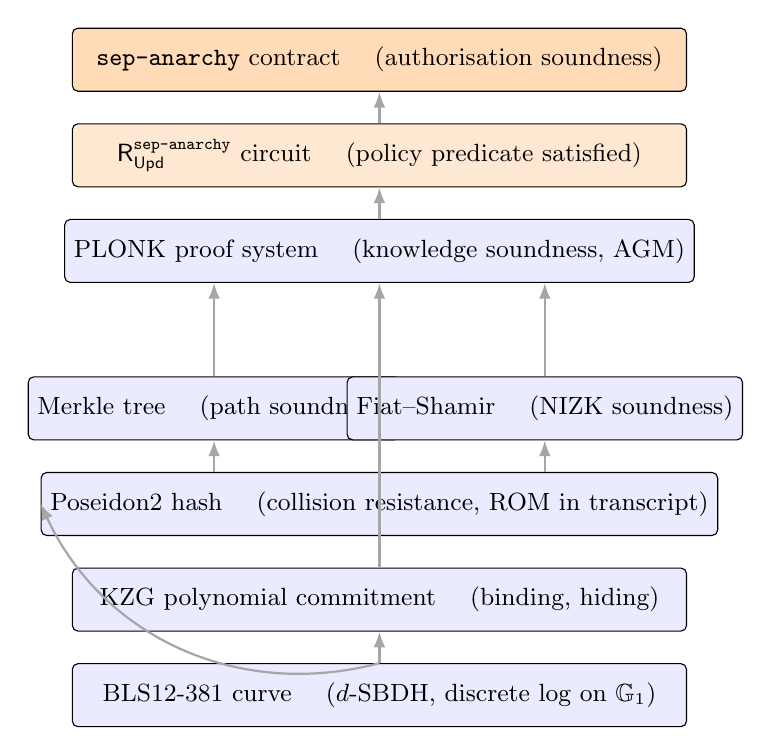
\begin{tikzpicture}[
   node distance=4mm,
   layer/.style={draw,rounded corners=2pt,minimum width=78mm,minimum height=8mm,align=center,font=\small},
   dep/.style={-{Latex[length=2mm]},thick,gray!70},
]
\node[layer,fill=blue!8] (curve) at (0,0)
   {BLS12-381 curve \quad ($d$-SBDH, discrete log on $\Gone$)};
\node[layer,fill=blue!8,above=of curve] (kzg)
   {KZG polynomial commitment \quad (binding, hiding)};
\node[layer,fill=blue!8,above=of kzg] (p2)
   {Poseidon2 hash \quad (collision resistance, ROM in transcript)};
\node[layer,fill=blue!8,above=of p2,minimum width=37mm,xshift=-21mm] (merkle)
   {Merkle tree \quad (path soundness)};
\node[layer,fill=blue!8,above=of p2,minimum width=37mm,xshift=21mm] (fs)
   {Fiat--Shamir \quad (NIZK soundness)};
\node[layer,fill=blue!8,above=24mm of p2] (plonk)
   {PLONK proof system \quad (knowledge soundness, AGM)};
\node[layer,fill=orange!18,above=of plonk] (rupd)
   {$\RUpd^{\sep{anarchy}}$ circuit \quad (policy predicate satisfied)};
\node[layer,fill=orange!28,above=of rupd] (sep)
   {\sep{anarchy} contract \quad (authorisation soundness)};

\draw[dep] (curve.north) -- (kzg.south);
\draw[dep] (kzg.north) -- (plonk.south);
\draw[dep] (curve.north) to[bend left=40] (p2.west);
\draw[dep] (p2.north -| merkle.south) -- (merkle.south);
\draw[dep] (p2.north -| fs.south) -- (fs.south);
\draw[dep] (merkle.north) -- (plonk.south -| merkle.north);
\draw[dep] (fs.north) -- (plonk.south -| fs.north);
\draw[dep] (plonk.north) -- (rupd.south);
\draw[dep] (rupd.north) -- (sep.south);
\end{tikzpicture}
\caption{Dependency stack. Each arrow is one reduction; the
contract (top) is authorisation-sound iff every layer below
holds. The diagonal arrow from BLS12-381 to Poseidon2 marks that
Poseidon2 is defined over the curve's scalar field $\Fr$; it is
not a soundness reduction but a parameter-set choice.}
\label{fig:chain}
\end{figure}

\section{Post-quantum considerations}
\label{sec:pq}

The base assumptions of \Cref{thm:auth} differ sharply in how
they fare against a cryptographically-relevant quantum computer
(CRQC). We delineate them explicitly because the composition is
only as strong as its weakest assumption.

Shor's algorithm~\cite{shor-1994-quantum} recovers discrete
logarithms in any abelian group in polynomial time on a CRQC,
including the source subgroups $\Gone, \Gtwo$ of BLS12-381. This
collapses \Cref{ass:sbdh}: the SRS becomes a full-knowledge
witness for the adversary, who can extract the trapdoor $\tau$
directly from the elements $[\tau^i]_1, [\tau^i]_2$. KZG
binding follows (\Cref{lem:kzg}), then PLONK knowledge
soundness (\Cref{lem:plonk-se}), then \Cref{thm:auth}. The stack
fails simultaneously at the curve layer.

Grover's algorithm gives a quadratic speedup on generic search,
halving the bit-security of preimage and collision resistance
for hash functions. \Cref{ass:p2cr} and \Cref{ass:p2rom} survive a
CRQC with reduced security margins ($128$-bit classical
collision resistance becomes roughly $64$-bit post-quantum) but
do not collapse; the Merkle and Fiat--Shamir layers
(\Cref{lem:merkle,lem:fs}) inherit this degradation without
losing their qualitative soundness.

\begin{proposition}
Under a CRQC, \Cref{thm:auth} fails through the curve layer
alone: \Cref{ass:sbdh} no longer holds, and the chain of
reductions breaks at \Cref{lem:kzg}. The hash-based layers
above continue to satisfy their respective reductions with
halved bit-security margins, but those reductions are no
longer load-bearing because the consumer
(\Cref{lem:plonk-se}) has already failed.
\end{proposition}

A post-quantum variant of the contract requires substituting the
proof system: a hash-based SNARK (FRI / STARKs) or a lattice-based
SNARK would replace PLONK, KZG, and the trusted-setup
assumption simultaneously. The Merkle commitment, the Poseidon2
hash, and the Fiat--Shamir transcript would be reused with no
qualitative change to \Cref{thm:auth}'s structure --- only the
proof-system reduction would change shape. We do not pursue this
substitution here.

\section{Implementation discipline the proof depends on}
\label{sec:notes}

\Cref{thm:auth} is conditional on several operational practices
that are easy to state and easy to get wrong. We list them
explicitly.

\paragraph{Domain separation in Fiat--Shamir.} The transcript
must open with a context tag binding the relation name, the
verifying-key digest, and any tier-index parameter that
distinguishes circuits. Two circuits sharing the same Poseidon2
instance without distinct tags would let an adversary transplant
a challenge derived in one transcript into another, defeating
the soundness loss of \Cref{lem:fs}.

\paragraph{Public-input absorption order.} Every public input
($\Cg$, $\Cgp$, the epoch, the policy tag) must be absorbed into
the transcript \emph{before} any verifier challenge is drawn from
it. Missing absorptions admit proof-malleability attacks in
which an adversary rewrites a public input in flight without
invalidating the proof; published deployment postmortems
document the operational cost of getting this
wrong~\cite{don-2019-fiat-shamir}.

\paragraph{SRS provenance.} The reused KZG ceremony output must
be hash-chained into the verifying-key supply chain using a
collision-resistant hash distinct from the in-circuit one
(SHA-256, in the deployment here~\cite{nist-fips-180-4}). The
verifying-key hash binds every published verifier to the exact
SRS bytes produced by the ceremony; otherwise the
one-honest-contributor assumption is not portable to the
verifying side.

\paragraph{Tier choice locked at group creation.} A group's
Merkle depth is fixed at creation time; growing the membership
set past the tier's bound requires migrating to a larger-tier
contract, not patching the deployed one. The proof of
\Cref{thm:auth} treats $D$ as a fixed parameter; a dynamic $D$
would require revisiting \Cref{lem:merkle}.

\paragraph{Policy predicate scope.} The proof here is for
\sep{anarchy}'s minimum predicate. The other policies in the
family substitute richer predicates inside $\RUpd$, but the
predicate's content does not enter \Cref{lem:plonk-se} or any layer
below: it appears only in the final reduction step (the policy
predicate inside $\RUpd^{\mathrm{policy}}$ implies the
contract's authorisation property). \Cref{cor:family} therefore
applies as long as the predicate is correctly compiled and the
compilation is verified against the verifying-key digest.

\paragraph{Identity uniqueness is not enforced by the predicate.}
\Cref{def:rupd} constrains $\ell^{\star}$ to be non-empty but
does not require that $\ell^{\star}$ differ from any leaf already
present in $\Cg$. A current member may therefore admit a value
that already occurs elsewhere in the tree, or two distinct values
that share an underlying identity key (with different blinding
factors). This is intrinsic to the \sep{anarchy} predicate ---
``any current member admits any leaf'' --- and is by construction.
Deployments that require one-identity-per-member must either
enforce uniqueness out-of-band (e.g., via an external nullifier
set) or compile a richer predicate that carries a non-membership
witness for $\ell^{\star}$. The latter requires a sparse-Merkle or
indexed-Merkle variant, since binary Merkle non-membership is not
$O(\log n)$.

\paragraph{Bootstrap is outside the proof scope.}
\Cref{thm:auth} conditions on a non-empty initial commitment
$\Cg$: at least one leaf $\ell_a$ must already be present for any
admission to verify. How that initial leaf is installed --- via a
genesis transaction, a founder signature, or a dedicated
\texttt{create\_group} contract method --- is a separate
authorisation question that this paper does not analyse. A
deployment must publish the bootstrap construction alongside the
soundness statement; ad-hoc initial-root selection by an untrusted
party voids \Cref{thm:auth}.

\paragraph{Verifying-key supply chain.}
The threat model (\Cref{sec:threat}) grants $\Adv$ read-only
access to the deployed verifying keys. \Cref{thm:auth} therefore
conditions on the on-chain $\mathsf{vk}$ being the one produced
by preprocessing the canonical \sep{anarchy} $\RUpd$ circuit
under the Ethereum Foundation KZG SRS. A maliciously-deployed
verifying key that uses an alternative SRS for which the deployer
knows $\tau$ admits proofs that the contract accepts but which
are unsound under the EF SRS. Users must verify the on-chain
$\mathsf{vk}$ against the SHA-256 digest published with the
release artifact; the digest verification is the user's
responsibility, not the chain's, and the soundness theorem is
silent on what happens when it is omitted.

\paragraph{Epoch monotonicity is chain-state, not a circuit
invariant.} \Cref{def:rupd} does not constrain the epoch $e$ in
its predicate body: $e$ is a public input bound into the
Fiat--Shamir transcript --- so an accepted proof attests to a
specific epoch value --- but the predicate itself imposes no
arithmetic relation among epoch values. Monotonicity (each
admission strictly increases $\mathsf{self.epoch}$ by exactly one)
is enforced by the on-chain contract, which passes the current
epoch as the public input and increments stored state on success.
Sequential composition (\Cref{rem:seq}) is therefore conditional
on the chain providing a total ordering of transactions; chain
reorganisations are a chain-level concern and outside the
cryptographic scope.

\section{Conclusion}
\label{sec:conclusion}

We presented a self-contained compositional sketch of the
authorisation-soundness chain for the simplest membership-policy
contract in a SNARK-gated group registry. Each layer of the
cryptographic stack contributes a single reduction; composing
them gives a top-level soundness statement that is fully
auditable against a small set of base assumptions: $d$-SBDH on
BLS12-381, collision resistance of Poseidon2 at its published
parameters, the random-oracle modelling of Poseidon2 inside the
transcript, and the one-honest-contributor assumption of the
reused structured reference string.

Two structural points are load-bearing and easy to miss. First,
the update relation requires \emph{two} Merkle witnesses --- one
for the admitter's membership, one for the target slot's
emptiness, with index distinctness between them. A naive
single-witness relation would permit a current member to overwrite
their own slot rather than genuinely admit a new member; the
two-witness shape rules this out (\Cref{rem:slot}). Second, the
proof-system reduction is the simulation-extractable strengthening
of plain knowledge soundness (\Cref{rem:se-vs-ks}); plain
knowledge soundness is insufficient against an adversary that
observes a polynomial history of accepted proofs on chain. The
strengthening is established for PLONK with updatable SRS under
the Fiat--Shamir absorption discipline catalogued in
\Cref{sec:notes}.

We made explicit which assumption fails first under a CRQC, and
we listed the operational practices the proof is conditional on
--- bootstrap, verifying-key supply chain, and chain-level
sequential composition. The result is a checklist of what must
hold for the deployment to be authorisation-sound, and a precise
statement of the boundary between the part of the stack that
survives Shor and the part that does not.

\bibliographystyle{plain}
\bibliography{references}

\end{document}
